\chapter{Evaluation de l'efficacité du Neurofeedback par la méta-analyse}

\section*{Introduction}
Les méta-analyses ont pour but de combiner les données de plusieurs études visant à démontrer l'efficacité d'un traitement. Cette méthode est
particulièrement intéressante lorsque les études comportent un faible nombre de sujets, comme c'est notamment le cas dans la plupart de celles sur 
le \gls{nfb} appliqué aux enfants \gls{tdah}.

Les différentes étapes à suivre pour réaliser une méta-analyse sont détaillées dans ce chapitre et résumées en Figure~\ref{Figure:pipeline_meta_analyse}.
Ces étapes sont ensuite appliquées à la réplication et à la mise à jour d'une récente méta-analyse sur le \gls{nfb} appliqué aux enfants \gls{tdah}, 
celle de \citet{Cortese2016}, dont certains résultats ont été débattus par la communauté scientifique \citep{Micoulaud2016}. Ainisi, cette analyse a pour but
de mettre en évidence l'impact de certains choix de \citet{Cortese2016} sur ses conclusions quant à l'efficacité du \gls{nfb}
\clearpage

\section{Principe d'une méta-analyse} \label{methods}

Les différentes étapes pour réaliser une méta-analyse sont décrites dans cette partie. Bien qu'il existe des logiciels permettant de réaliser une
méta-analyse, ces étapes ont été implémentées en Python par souci de transparence et de reproductibilité dont le code source est disponible sur un dépôt GitHub \citep{Bussalb2019c}.

\subsection{Buts d'une méta-analyse}

Les méta-analyses rassemblent les résultats de plusieurs études, satisfaisant des critères d'inclusion préalablement établis, dans le but d'analyser
sur un plus grand nombre de sujets provenant de populations différentes, l'efficacité d'un traitement. Alors qu'avant les années 1990 les revues narratives
(\textit{narrative reviews} en anglais) étaient le plus couramment utilisées pour cette tâche, elles ont perdu leur popularité au profit des méta-analyses.
En effet, les revues narratives souffrent de la subjectivité des auteurs qui choisissent notamment le poids à donner à telle ou telle étude : alors que certains
vont donner plus d'importance aux études incluant de nombreux sujets, d'autres vont favoriser les études qu'ils jugent de bonne qualité. La méta-analyse permet 
de réduire cette subjectivité en utilsant par exemple des critères mathématiques définis à l'avance pour calculer le poids à attribuer à chaque étude incluse
\citep{Borenstein2009}.

Réaliser une méta-analyse permet de confronter les résultats de toute étude incluse à ceux des autres études intégrées dans l'analyse : l'efficacité (mesurée par 
une valeur standardisée appelée taille d'effet ou \gls{es} en anglais) est-elle constante parmi l'ensemble des études sélectionnées ? 
Auquel cas, l'\gls{es} doit être calculé précisément, sinon on cherche à quantifier à quel point l'efficacité entre les études varie.

\subsection{Choix du modèle}

La première étape consiste à choisir le modèle statistique de la méta-analyse. La plupart des méta-analyses sont basées sur l'un des deux modèles 
suivants qui reposent sur des hypothèses scientifiques différentes \citep{Borenstein2009} :
\renewcommand{\labelitemi}{$\bullet$}
\begin{itemize}
\item le modèle à effet fixe (\textit{fixed-effect model} en anglais),
\item le modèle à effets aléatoires (\textit{random-effects model} en anglais).
\end{itemize}

Dans le cas du modèle à effet fixe, il est supposé qu'il existe un \gls{es} réel (\textit{true} \gls{es} en anglais), c'est à dire l'\gls{es} qui serait
observé avec un nombre de sujets infiniment grand, qui serait le même pour l'ensemble des études incluses dans la méta-analyse. Les différences entre
les \gls{es} observés pour chaque étude sont dues à des erreurs d'échantillonnage. Au contraire, dans le cas du modèle à effets aléatoires, 
l'\gls{es} réel peut varier entre les études. Cette variabilité s'explique non seulement par des erreurs d'échantillonnage mais aussi par 
les différentes conceptions des études et/ou par les différences entre les sujets inclus.

L'hypothèse nulle testée lors de la méta-analyse est différente selon le modèle choisi :
\begin{itemize}
\item pour le modèle à effet fixe : 
\textit{$H_{0}$ : le traitement n'a auncun effet dans chaque étude},
\item pour le modèle à effets aléatoires : 
\textit{$H_{0}$ : l'effet moyen du traitement est nul}.
\end{itemize}

Le modèle à effets aléatoires est souvent plus approprié du fait de la variabilité des études. En effet, même si les études incluses dans la méta-analyse 
répondent toutes aux critères d'inclusion fixés au préalable, rien ne peut généralement permettre de supposer que ces études sont identiques et qu'elles 
partagent donc toutes le même \gls{es} réel. Le modèle à effet fixe est ainsi rarement utilisé, on peut cependant y avoir recours lorsque le nombre d'études inluses 
est très petit. Au sein du domaine du \gls{nfb} appliqué aux enfants \gls{tdah}, les méta-analyses suivent le modèle à effets aléatoires 
\citep{Cortese2016, Micoulaud2014}, c'est donc ce modèle que nous choisissons également.

\subsection{Calcul de la taille d'effet}

Une fois le modèle choisi, l'étape suivante est de quantifier l'efficacité de chaque étude incluse dans la méta-analyse en calculant son \gls{es}. 
Il existe différents \gls{es} \citep{Borenstein2009} :
\renewcommand{\labelitemi}{$\bullet$}
\renewcommand{\labelitemii}{$\cdot$}
\begin{itemize}
\item \gls{es} basés sur des moyennes :
\begin{itemize}
    \item la différence moyenne non standardisée (\textit{unstandardized mean difference} en anglais),
    \item la différence moyenne standardisée (\textit{standardized mean difference} en anglais).
\end{itemize}
\item \gls{es} basés sur des données binaires :
\begin{itemize}
    \item le taux de risque (\textit{risk ratio} en anglais),
    \item le taux de chance (\textit{odds ratio} en anglais),
		\item la différence de risque (\textit{risk difference} en anglais).
\end{itemize}
\end{itemize}

Etant donné que les données que nous allons utilisées pour la réplication et la mise à jour de \citet{Cortese2016} sont les moyennes des 
scores cliniques obtenus par les sujets sur des échelles évaluant les symptômes du \gls{tdah} avant le traitement (pré-test) et 
après le traitement (post-test) et leur écart-type, nous nous concentrons sur 
les \gls{es} basés sur des moyennes. Par ailleurs, les échelles cliniques variant 
d'une étude à l'autre, les moyennes ne sont pas comparables : il faut donc standardiser l'\gls{es}. 
Ainsi, nous allons utiliser la différence moyenne standardisée \citep{Cortese2016, Micoulaud2014}.

Enfin, lorsqu'un groupe contrôle est disponible, on peut calculer l'\gls{es}-inter-groupes (\textit{between}-\gls{es}) comme défini dans \citet{Morris2008}.
Cet \gls{es} est utilisé par \citet{Cortese2016, Micoulaud2014} et implémenté dans \citet{Bussalb2019} :
\begin{equation}
\label{eq:metareview_effect_size_between}
\text{ES-inter-groupes} = c_p \left(\frac{(M_{\text{post},T} - M_{\text{pre},T}) - (M_{\text{post},C} - M_{\text{pre},C}) }{\sigma_{\text{pre}}} \right).
\end{equation} 
L'\gls{es}-inter-groupes est équivalent au z-score d'une distribution normale. Il correspond à la différence entre la moyenne à post-test et à pré-test 
dans le groupe qui reçoit le traitement ($M_{\text{pre},T}$, $M_{\text{post},T}$) moins la différence entre la moyenne du score à post-test et à pré-test 
dans le groupe contrôle ($M_{\text{pre},C}$, $M_{\text{post},C}$), divisée par la \textit{pooled} standard deviation à pré-test ($\sigma_{\text{pre}}$) :
\begin{equation}
\label{eq:stats_metareview_std_pre}
\sigma_{\text{pre}} = \sqrt{\frac{(n_T - 1)\sigma_{\text{pre},T}^2 + (n_C - 1)\sigma_{\text{pre},C}^2} {n_T + n_C - 2}},
\end{equation}
où $\sigma_{t,G}$ correspond à l'écart-type du groupe $G$ à pré-test and $n_G$ indique le nombre de sujets dans chaque groupe ; 
$c_p$ est un bias d'ajustement utilisé pour les petites études :
\begin{equation}
\label{eq:metareview_correction_factor}
c_p =  1 - \frac{3} {4(n_T + n_C - 2) - 1}. 
\end{equation} 

\subsection{Calcul de la précision de chaque taille d'effet}

Le terme précision englobe trois valeurs statistiques liées les unes aux autres : la variance, l'erreur standard, et l'intervalle de confiance.
Ces trois facteurs de précision définissent un intervalle de valeurs probables pour l'\gls{es} réel. 

Tout d'abord, la variance de chaque \gls{es}-inter-groupes est calculée \citep{Morris2008}:
\begin{equation}
\label{eq:metareview_variance_effect_size_between}
\sigma^2(\text{ES}) = c_p^2 \left (\frac{n_T + n_C - 2} {n_T + n_C - 4} \right ) \left  (\frac{2(1-r)(n_T + n_C)} {n_Tn_C} + \text{ES}^2 \right) - \text{ES}^2,
\end{equation}
où \gls{es} désigne l'\gls{es}-inter-groupes et $r$ la \textit{pooled} corrélation de Pearson intra-groupes \citep{James2013} :
\begin{equation}
\label{eq:metareview_within_group_pearson_correlation}
r = \frac{ \sum_{i=1}^{n} (\text{pre}_i - \mu_{\text{pre}})(\text{post}_i - \mu_{\text{post}}) } { \sqrt{ \sum_{i=1}^{n} (\text{pre}_i - 
\mu_{\text{pre}})^2} \sqrt{\sum_{i=1}^{n} (\text{post}_i - \mu_{\text{post}})^2} }, 
\end{equation}
où $n$ est le nombre de patients inclus dans une étude, $\text{pre}_i$, $\text{post}_i$ les valeurs de scores cliniques pour le sujet $i$ 
respectivement à pré- et post-test, et $\mu_{\text{pre}}$, $\mu_{\text{post}}$ les scores moyens calculés sur tous les sujets. 
Il s'agit d'une mesure de corrélation linéaire entre deux variables : une valeur de 1 signifie une corrélation positive entre ces variables,
une valeur de -1 une corrélation négative, et une valeur de 0 une absence de corrélation linéaire. 
Dans notre cas, cette corrélation étant inconnue et les données brutes n'étant pas disponibles, nous approximons la valeur de $r$ 
en accord avec \citet{Balk2012}, qui a trouvé qu'une valeur de 0.5 conduit à des résultats proches de ceux obtenus avec la véritable
valeur de la corrélation.

Une fois la variance obtenue, il est aisé de calculer l'\gls{et} (\textit{standard error} en anglais) de l'\gls{es}-inter-groupes 
\citep{Borenstein2009} :
\begin{equation}
\label{eq:metareview_standard_error_effect_size_between}
\text{ET} = \sqrt{\sigma^2(\text{ES})},
\end{equation}
où \gls{es} désigne l'\gls{es}-inter-groupes. Alors que la variance est intéressante pour les calculs statistiques, l'\gls{et} est quant à elle 
un index plus aisé à comprendre car elle est sur la même échelle que l'\gls{es}.

Enfin, si l'\gls{es}-inter-groupes suit une distribution normale, l'intervalle de confiance à 95\% peut être calculé \citep{Borenstein2009}.

La précision est affectée dans une large mesure par le nombre de sujets inclus dans l'étude : les échantillons plus grands mènent à des
estimations de \gls{es}-inter-groupes plus précises, c'est pourquoi un plus grand poids leur est attribué dans la méta-analyse.

\subsection{Calcul de l'effet total du traitement}

Afin d'obtenir l'estimation la plus précise possible de l'effet du traitement sur la population, une moyenne pondérée des \gls{es}-inter-groupes 
des études incluses est calculée.

Si le modèle à effet fixe est choisi, le poids $w_{\text{fixe}_k}$ assisgné à chaque étude $k$ correspond à l'inverse de la variance de son 
\gls{es}-inter-groupes ($\sigma^2(\text{ES})$, la variance intra-étude) \citep{Borenstein2009} :
\begin{equation}
\label{eq:metareview_weight_fixed_study}
w_{\text{fixe}_k} = \frac{1}{\sigma^2(\text{ES}_k)}.
\end{equation} 

Dans notre cas nous employons le modèle à effets aléatoires \citep{Bussalb2019}, qui inclut également la variance inter-études $\tau^2$ conduisant à des 
poids ($w_{\text{aléatoires}_k} = w_k$) associés aux études dfférents.

Calculer la variance inter-études se fait en trois étapes décrites par les équations Eq.~(\ref{eq:metareview_Q}), Eq.~(\ref{eq:metareview_C}) 
et Eq.~(\ref{eq:metareview_Tau}) \citep{Borenstein2009} :
\begin{equation}
\label{eq:metareview_Q}
Q = \sum_{k=1}^{K} (w_{\text{fixe}_k} \text{ES}_k^2),
\end{equation}
\begin{equation}
\label{eq:metareview_C}
C = \sum_{k=1}^{K} w_{\text{fixe}_k} - \frac{ \sum_{k=1}^{K} (w_{\text{fixe}_k})^2 } { \sum_{k=1}^{K} w_{\text{fixe}_k} },
\end{equation}
avec $K$ le nombre total d'études incluses.
\begin{equation}
\label{eq:metareview_Tau}
\tau^2 = \frac{Q - \text{df}}{C},
\end{equation}
avec $\text{df} = K - 1$ le degré de liberté.

Le modèle à effets aléatoires prenant en compte les différences entre les études, les poids sont égaux à l'inverse de la somme entre la variance intra-étude
$\sigma^2(\text{ES}_k)$ et la variance inter-études $\tau^2$ \citep{Borenstein2009} :
\begin{equation}
\label{eq:metareview_weight_study}
w_k = \frac{1}{\sigma^2(\text{ES}_k) + \tau^2}.
\end{equation} 

Enfin, la moyenne pondérée des $K$ \gls{es}-inter-groupes est calculée pour obtenir l'\gls{est} comme décrit dans l' 
Eq.~(\ref{eq:metareview_summary_effect}) \citep{Borenstein2009}:
\begin{equation}
\label{eq:metareview_summary_effect}
\text{EST} = \frac{\sum_{k=1}^{K} w_k \text{ES}_k} {\sum_{k=1}^{K} w_k}.
\end{equation} 
Une fois le \gls{est} obtenu, on peut calculer sa variance, son erreur type, son intervalle de confiance à 95\%, sa p-value, 
et $I^2$ qui estime l'hétérogénéité des \gls{es}-inter-groupes. 

\subsection{Répresentation graphique des résultats d'une méta-analyse}

Afin de faciliter la lecture des résultats d'une méta-analyse, ceux-ci sont résumés dans un \textit{forest plot} \citep{Borenstein2009}. Les études incluses sont
en ordonnées et les \gls{es}-inter-groupes en abscisses. Chaque \gls{es}-inter-groupes est représenté par un carré dont la taille est proportionnelle
au poids $w_k$ attribué à l'étude $k$. Les intervalles de confiance à 95\% pour chaque \gls{es}-inter-groupes sont représentés. En bas du graphique, l'\gls{est}
est symbolisé par un diamant avec son intervalle de confiance à à 95\%. Une droite verticale d'équation $x = 0$ est tracée pour délimiter la
partie du graphique où les \gls{es} sont en faveur du traitement de celle où ils ne le sont pas.

Un autre graphique très utilisé dans la méta-analyse est le \textit{funnel plot} qui a pour but de détecter un éventuel biais de publication
lors de la sélection des études et une hétérogénéité parmi elles \citep{Sterne2011}. Il s'agit d'un nuage de points de la précision de chaque 
\gls{es}-inter-groupes en fonction des \gls{es}-inter-groupes. L'inverse de l'\gls{et} est couramment utilisé comme estimation de la précision et de la 
taille d'une étude et est placé sur un axe des abscisses inversé de façon à ce que les plus grandes études soient au sommet et que les plus petites se retouvent 
dispersées en bas. En l'absence de biais et d'hétérogénéité entre les études, la répartition des points est seulement due à la variabilité de la taille des études : 
le graphique est symétrique. Le triangle centré sur \gls{est} obtenu avec un modèle à effet fixe et s'étendant de 1.96 \gls{et} de chaque côté 
inclut 95\% des études s'il n'y a pas de biais.

Déterminer l'asymétrie d'un \textit{funnel plot} peut se faire visuellement mais aussi mathématiquement en utilisant par exemple le test de \citet{Egger1997}. 
Il s'agit de regresser les \gls{es}-inter-groupes divisés par leur \gls{et} sur l'inverse des \gls{et}. Si l'intercept diffère significativement de 
0 (seuil de signifiance à 0.05) alors le \textit{funnel plot} est asymétrique.

L'ensemble des étapes pour réaliser une méta-analyse en suivant le modèle à effets aléatoires est résumé à la Figure~\ref{Figure:pipeline_meta_analyse}.

\begin{figure}[h!]
  \centering
	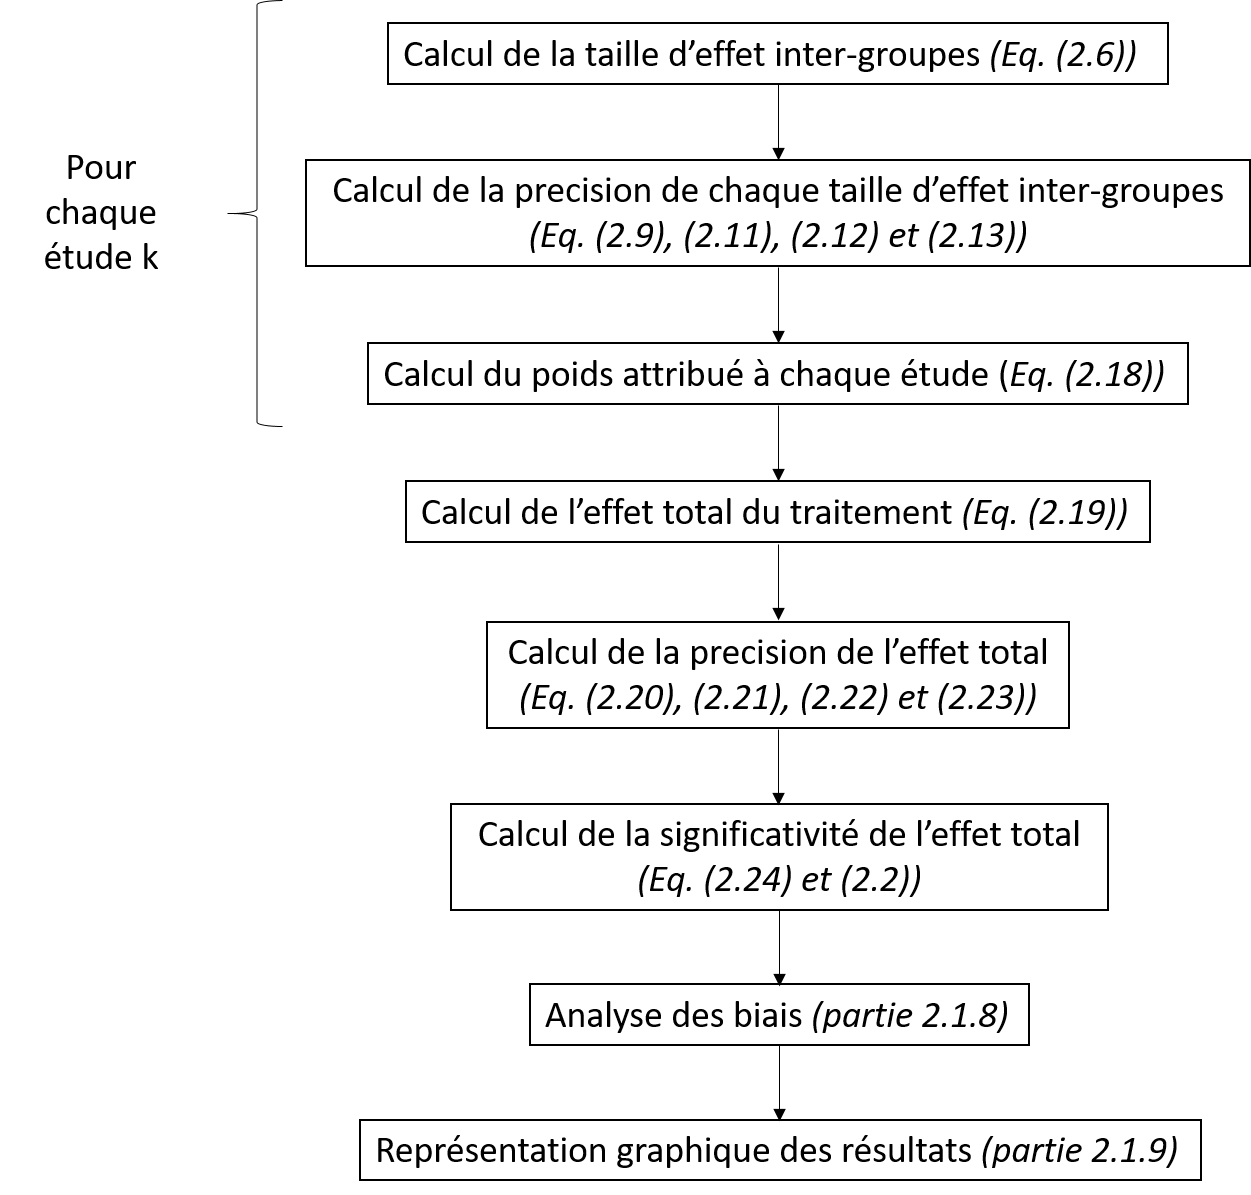
\includegraphics[width=1.0\linewidth]{figures/chapter-2/pipeline-perform-meta-analysis} 
  \caption{Résumé des étapes à suivre pour effectuer une méta-analyse dans le cadre d'un modèle à effets aléatoires.}
  \label{Figure:pipeline_meta_analyse}
\end{figure}

\section{Replication et mise à jour de la méta-analyse de Cortese et al., 2016} \label{replication_and_update}

La méta-analyse de \citet{Cortese2016} a eu un fort impact dans la communauté du \gls{nfb}, d'une part du fait du nombre d'études incluses (13) et d'autre part
du fait du soin apporté au choix des études. Cependant, quelques choix faits par les auteurs, comme le souligne \citet{Micoulaud2016} méritent d'être explorés.
C'est pourquoi dans un premier temps, la méta-analyse de \citet{Cortese2016} est répliquée en modifiant les points débattus pour évaluer leur impact sur les
résultats. Ensuite, étant donné que la recherche dans le domaine du \gls{nfb} appliqué aux enfants \gls{tdah} est très active, de nouvelles études ont pu
être publiées depuis la méta-analyse de \citet{Cortese2016} et qui aurait pu y être incluses. La mise à jour de ce genre d'analyse est importante
car plus d'études y seront incluses plus les résultats vont se stabiliser, c'est pourquoi nous allons relancer l'analyse avec les nouvelles études
satisfaisant les critères d'inclusion de \citet{Cortese2016}.

Dans un souci de transparence et pour faciliter la réplication de ce travail, ces deux analyses sont effectuées en utilisant le package Python dont 
le contenu est décrit en \ref{methodes} \citep{Bussalb2019c}. 

\subsection{Réplication de la méta-analyse de Cortese et al., 2016}

\subsubsection{Evaluation des résultats obtenus avec le package Python}

Tout d'abord, avant de discuter de certains choix de \citet{Cortese2016}, le package Python ayant pour but de réaliser une méta-analyse est évalué
en répliquant exactement ce qui a été fait dans \citet{Cortese2016}. 

Pour effectuer une méta-analyse, les auteurs utilisent en général le logiciel RevMan \citep{Revman}. Ici les résultats obtenus avec le package Python vont être
comparés à ceux donnés par la version 5.1 de RevMan. 

La première étape a été d'entrer dans un fichier .csv pour chaque étude incluse les scores cliniques à pré-test et post-test avec leur écart-type utilisés 
par \citet{Cortese2016} pour calculer les \gls{es}-inter-groupes. Lorsqu'ils sont disponibles les scores cliniques évaluant l'inattention, l'hyperactivité 
et la totalité des symptômes sont extraits afin d'obtenir une valeur d'efficacité sur chacune de ces composantes. Par ailleurs, les scores donnés par les
parents mais aussi par les enseignants sont utilisés : ce qui différencie ces deux types d'évaluateurs est leur connaissance du traitement. Alors que les
parents connais

Une fois cette étape remplie, le package Python lit ce fichier et retourne l


\subsection{Mise à jour de la méta-analyse de Cortese et al., 2016}

\section{Discussion sur l'hétérogénéité des études} 